\documentclass[10pt]{article}
\usepackage[utf8]{inputenc}
\usepackage[T1]{fontenc}
\usepackage{graphicx}
\usepackage[export]{adjustbox}
\graphicspath{ {./images/} }
\usepackage{amsmath}
\usepackage{amsfonts}
\usepackage{amssymb}
\usepackage{mhchem}
\usepackage{stmaryrd}
\usepackage{bbold}

\begin{document}
\subsection{D and 2D Finite Element and Multigrid}
1D and 2D Comparison for Finite Element and Multigrid

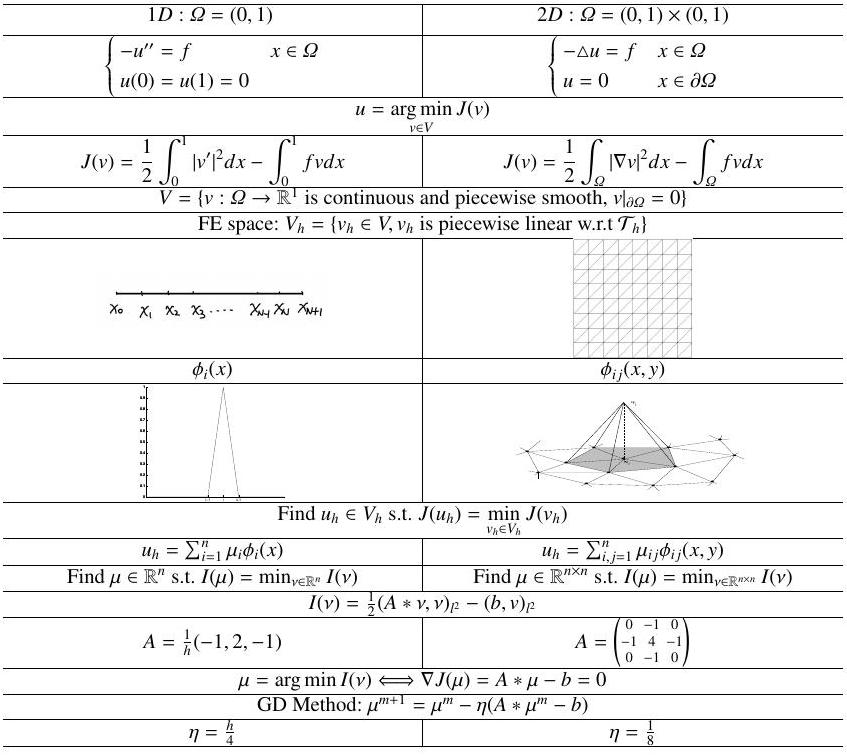
\includegraphics[max width=\textwidth]{2022_01_06_175a66d2121dcf20361ag-1}

Basic multigrid components

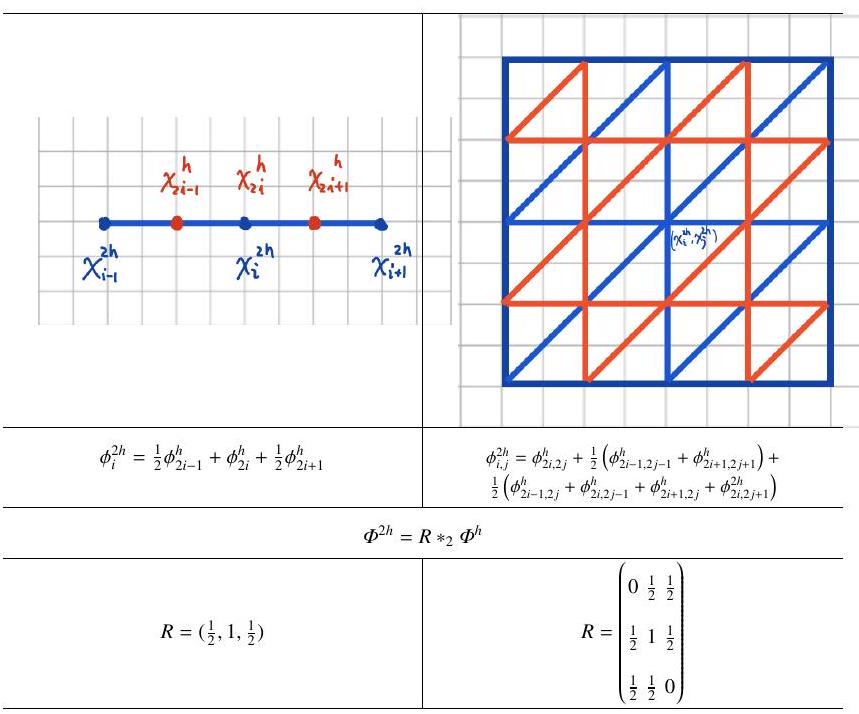
\includegraphics[max width=\textwidth]{2022_01_06_175a66d2121dcf20361ag-2}

\subsubsection{Multigrid algorithm for $A * \mu=f$}
\section{Algorithm 11 A multigrid algorithm $\mu=\operatorname{MG} 1\left(f ; \mu^{0} ; J, v_{1}, \cdots, v_{J}\right)$ 
 Set up}
$$
f^{1}=f, \quad \mu^{1}=\mu^{0}
$$
Smoothing and restriction from fine to coarse level (nested)

for $\ell=1: J$ do

for $i=1: v_{\ell}$ do
$$
\mu^{\ell} \leftarrow \mu^{\ell}+S^{\ell} *\left(f^{\ell}-A_{\ell} * \mu^{\ell}\right)
$$
end for

Form restricted residual and set initial guess:
$$
\mu^{\ell+1} \leftarrow \Pi_{\ell}^{\ell+1} \mu^{\ell}, \quad f^{\ell+1} \leftarrow R *_{2}\left(f^{\ell}-A_{\ell} * \mu^{\ell}\right)+A_{\ell+1} * \mu^{\ell+1},
$$
end for

Prolongation and restriction from coarse to fine level

for $\ell=J-1: 1$ do
$$
\mu^{\ell} \leftarrow \mu^{\ell}+R *_{2}^{\top}\left(\mu^{\ell+1}-\Pi_{\ell}^{\ell+1} \mu^{\ell}\right)
$$
end for
$$
\mu \leftarrow \mu^{1}
$$
Remark 9. The above multigrid method for the linear problem $A * \mu=b$ is independent of the choice of the interpolation operation $\Pi_{\ell}^{\ell+1}: \mathbb{R}^{n_{\ell} \times n_{\ell}} \mapsto \mathbb{R}^{n_{\ell+1} \times n_{\ell+1}}$ and in particular, we could take $\Pi_{\ell}^{\ell+1}:=0$. But such an operation is critical for nonlinear problems.

\subsubsection{MgNet}
Algorithm $12 \mu^{J}=\operatorname{MgNet} 1\left(f ; \mu^{0} ; J, v_{1}, \cdots, v_{J}\right)$
\[ \begin{array}{l}\text { Set up } \\ \qquad f^{1}=\theta * f, \quad \mu^{1}=\mu^{0} .\end{array} \]
Smoothing and restriction from fine to coarse level (nested)\\
for $\ell=1: J$ do $\quad$ for $i=1: v_{\ell}$ do\\
(8.34) $\quad \mu^{\ell} \leftarrow \mu^{\ell}+\sigma \circ S^{\ell} * \sigma \circ\left(f^{\ell}-A_{\ell} * \mu^{\ell}\right) .$\\
end for $\quad f^{\ell+1} \leftarrow \Pi_{\ell}^{\ell+1} \mu^{\ell}, \quad f^{\ell+1} \leftarrow R *_{2}\left(f^{\ell}-A_{\ell} * \mu^{\ell}\right)+A_{\ell+1} * \mu^{\ell+1}$,\\
Form restricted residual and set initial guess:\\
end for


\end{document}